\chapter{Studi Literatur}

Pada bab ini, akan diisi oleh studi literatur, hal-hal yang berkaitan dengan topik persoalan tugas akhir akan dipaparkan dalam bab ini guna untuk memberikan informasi mengenai dasar teori dan studi yang dipakai. Bab ini diharapkan membantu pembaca untuk mengerti dalam membaca penelitian tugas akhir ini.


\section{\textit{Service}}

\textit{Service} dapat diartikan sebagai sebuah teknologi atau cara kerja yang dapat digunakan untuk memberikan keuntungan ataupun menyelesaikan suatu pekerjaan. Selain itu \textit{service} juga dapat diartikan sebagai abstraksi dari sebuah proses bisnis. \parencite{osullivan2002}

Secara umum \textit{Service} Memiliki tiga fitur utama yaitu.
\begin{enumerate}
  \item \textit{Service} dapat melakukan sebuah aksi atau pekerjaan untuk orang lain,
  \item \textit{Service} adalah sebuah aset yang memiliki sebuah nilai yang dapat diturunkan dari penyedia ke pengguna,
  \item \textit{Service} dapat di bungkus pada service lainnya (sub-services),
\end{enumerate}

Untuk menggabungkan \textit{service}, terdapat dua cara yaitu agregasi dan komposisi. Agregasi memiliki pendekatan untuk menggabungkan dua atau lebih \textit{service} dan membuat satu \textit{entrypoint} untuk seluruh \textit{service} tersebut. Berbeda dengan komposisi, komposisi menggunakan pendekatan untuk mengintegrasikan seluruh sub-\textit{services} yang ada dengan cara membuat jalur komunikasi antar \textit{service} dan setiap \textit{service} memiliki hubungan tertentu dengan \textit{service} lainnya.

Interaksi pada sebuah \textit{service} haruslah minimal memiliki tiga elemen, \textit{service provider}, \textit{service requestor/client}, serta \textit{\textit{service registry}}, namun terdapat juga elemen ke empat pada beberapa kasus yaitu \textit{service broker}. Illustrasi dapat dilhat pada gambar \ref{fig:tiga-elemen-service}

\begin{figure}[ht]
  \centering
  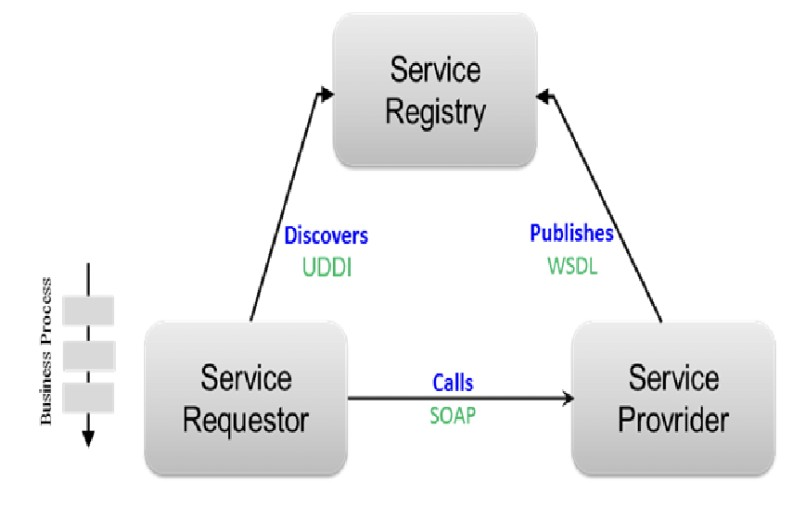
\includegraphics[width=0.8\textwidth]{chapter-2/tiga-elemen-service.jpg}
  \caption{Tiga Elemen pada Interaksi Service, \parencite{abugessaisa2023}}
  \label{fig:tiga-elemen-service}
\end{figure}

\textit{Service requestor} mengirimkan permintaannya serta kebutuhannya kepada \textit{service registry} untuk dicarikan service yang sesuai dengan kebutuhannya. Namun pada beberapa kasus khusus, \textit{service requestor}
sudah memiliki \textquotedblleft contract \textquotedblright dengan \textit{provider} tujuannya sehingga bisa langsung melakukan \textit{request} ke \textit{provider} tanpa bantuan dari \textit{service registry}.

Service \textit{provider} menyediakan \textit{service} yang dapat dikonsumsi oleh publik, agar \textit{service} nya dapat digunakan oleh requestor, \textit{service} \textit{provider} akan memberikan list \textit{services} yang dimiliki kepada registry untuk disimpan pada sebuah \textquotedblleft catalogue \textquotedblright yang dimiliki oleh registry.\textit{Service registry} berperan sebagai penengah dalam komunikasi \textit{requestor} dan \textit{provider}. \textit{Service registry} memiliki \textquotedblleft catalogue \textquotedblright yang menyimpan list berbagai macam \textit{service provider} yang dapat digunakan oleh \textit{service requestor}.

Dengan adanya ketiga elemen tersebut, interaksi pada \textit{services} dapat berjalan sehingga menciptakan suatu fungsionalitas seperti proses bisnis ataupun pemenuhan kebutuhan lainnya.


\section{\textit{Service Oritented Computing}}

Service oriented computing adalah sebuah paradigma yang memanfaatkan service sebagai dasar elemen untuk mengembangkan sebuah solusi dari permasalahan \parencite{papazoglou} 


\section{Evolusi\textit{Service Architecture}} 

\section{\textit{Service Mesh}}

\subsection{Definisi}

\textit{Service mesh} adalah sebuah infrastruktur yang memanage \textit{Service} komunikasi antar \textit{service}. \textit{Service mesh} dibuat dengan tujuan untuk memberikan layer tambahan untuk architecture yang dibuat tanpa harus membuat kode aplikasi pada setiap \textit{service} untuk berkomunikasi.\parencite{li2019} 

Jika terdapat dua buah \textit{service}, kedua \textit{service} tersebut harus membuat sebuah interface ataupun cara menghubungkan masing masing \textit{service} untuk berkomunikasi karena perlu adanya beberapa penyesuaian, seperti penyesuaian bahasa pemrograman karena mungkin saja kedua \textit{service} tersebut menggunakan bahasa pemrograman yang berbeda. 

Setiap \textit{service} juga perlu menyesuaikan cara dari setiap \textit{service} tersebut menerima dan mengirim request. Beberapa \textit{service} mungkin saja menggunakan gRPC untuk menerima dan mengirim request dan \textit{service} lain menggunakan REST ataupun graphQL. Bayangkan jika kita memiliki lebih dari 100 \textit{service} yang ingin ber orkestrasi dan berkomunikasi satu sama lain, kita harus membuat interface untuk setiap \textit{service} yang ada dan hal ini sangat memakan waktu.

\textit{Service mesh} hadir untuk menyelesaikan masalah ini terutama masalah komunikasi internal antar \textit{service}. Selain itu, \textit{Service mesh} juga memberikan fitur seperti \textit{service discovery}, \textit{central authentication}, \textit{access control}, \textit{load balancing}, \textit{logging}, serta \textit{monitoring}. Selain memberikan fitur tersebut, \textit{\textit{service} mesh} juga harus memiliki \textit{reliability} serta \textit{fault tolerance}. \parencite{li2019} 

\textit{Service mesh} pada umumnya memiliki dua plane, \textit{control plane} dan \textit{data plane}. \textit{control plane} merupakan sebuah tempat terpusat untuk mengontrol jaringan mulai dari \textit{service discovery}, \textit{logging dan monitoring}, ataupun menjaga \textit{service level agreement} (SLA) agar \textit{availability} dari \textit{service} yang ada memiliki nilai yang baik. \textit{data plane} sering disebut sebagai \textit{forwarding plane} karena bertujuan untuk meneruskan ataupun menerima request dari \textit{service} yang dituju sesuai arahan dari \textit{control plane}. Kedua \textit{plane} ini menjadi komponen paling penting dalam pembuatan \textit{\textit{service} mesh}.

Sudah banyak produk ataupun aplikasi yang menawarkan solusi untuk menyelesaikan masalah \textit{\textit{service} Mesh}, diantaranya Istio, Linkerd, Airbnb Synapse, dan AWS App Mesh. Keempat aplikasi tersebut memiliki cara tersendiri agar \textit{\textit{service} mesh} dapat berjalan dengan baik. Berikut tabel perbandingan dari keempat produk tersebut


\begin{longtable}{|p{1.5cm}|p{1.5cm}|p{1.5cm}|p{1.5cm}|p{1.5cm}|p{1.5cm}|p{1.5cm}|}
  \caption{Perbandingan aplikasi \textit{service mesh}} \label{tab:perbandingan-service-mesh} \\
  \hline
  \rowcolor{gray!30} \textbf{Aplikasi} & \textbf{\textit{Data plane}} & \textbf{\textit{Open source}} & \textbf{\textit{Activeness}} & \textbf{\textit{Major advantage}} & \textbf{\textit{Critical limitation}} & \textbf{\textit{Rating overall}} \\
  \hline
  \endfirsthead

  \endhead
  
  % \textit{Intelligent Workload Factoring for a Hybrid Cloud Computing Model}, \parencite{zhang} & VM & \textit{Request Rate} & Reaktif & ARIMA \tabularnewline
  Istio & Envoy & Yes & Good & Growing Community and Fast Iteration & Lack of support & Moderate \tabularnewline \hline

  Linkerd2 & Linkerd-proxy & Yes & Good & Stability and CNCF Accepted & Potential vendor Lock-in & Good \tabularnewline \hline

  AWS App Mesh & Envoy & No & Good & Native Compatibility with AWS & Closed Ecosystem & Preview \tabularnewline \hline

  Airbnb Synapse & HAProxy / Nginx & Yes & Poor & N/A & Limited Features & Poor \tabularnewline \hline

  % \textit{Autonomic Vertical Elasticity of Docker Containers with Elasticdocker}, \parencite{al2017autonomic} & \textit{Container} & Prosesor, Memori & Reaktif & \textit{Rule-based} \tabularnewline

  % \textit{Horizontal Pod Autoscaler}, \parencite{hpa2} & \textit{Container} & Prosesor & Reaktif & \textit{Rule-based} \tabularnewline

  % \textit{A Novel Resource Prediction and Provisioning Scheme in Cloud Data Center}, \parencite{rpps} & \textit{Container} & Prosesor & Proaktif & ARMA \tabularnewline

  % \textit{Workload Prediction Using ARIMA Model and Its Impact on Cloud Applications QoS}, \parencite{workloadprediction} & VM & \textit{Request Rate} & Proaktif & ARIMA \tabularnewline

  % \textit{Resource Elasticity Controller for Docker-based Web Applications}, \parencite{resourceelasticity} & \textit{Container} & \textit{Request Rate} & Proaktif & ARIMA \tabularnewline

  % \textit{Combining Time Series Prediction Models using Genetic Algorithm to Autoscaling Web Applications Hosted in the Cloud Infrastructure}, \parencite{tspwithga} & - & \textit{Request Rate} & Proaktif & \textit{Genetic Algorithm} \tabularnewline

  % \textit{Predicting Cloud Resource Provisioning using Machine Learning Techniques}, \parencite{predictcloudrsrc} & - & \textit{Task Length} & Proaktif & \textit{Artificial Neural Network} \tabularnewline

  % \textit{Auto-scaling Microservices on IaaS under SLA with Cost-Effective Framework}, \parencite{asmicrocosteff} & VM & \textit{Request Rate} & Proaktif & \textit{Artificial Neural Network}, \textit{Recurrent Neural Network} \tabularnewline

  % \textit{Machine Learning-based Auto-scaling for Containerized Applications}, \parencite{mlbasconapps} & \textit{Container} & \textit{Request Rate} & Proaktif & LSTM \tabularnewline

  % \textit{Adaptive Horizontal Scaling of Microservices using Bi-LSTM}, \parencite{adaptivehsmicro} & \textit{Container} & Prosesor, Memori & Gabungan & Bi-LSTM \tabularnewline

  \hline
\end{longtable}

\subsection{Interaksi}

Terdapat beberapa jenis interaksi yang dapat dilakukan pada service mesh diantaranya \parencite{ganguli2021}

\begin{enumerate}
  \item \textit{Pod to pod communication }
  \item \textit{Pod to service communication}
  \item \textit{Ingress controller to pod and vice-versa} 
  \item \textit{Load balancer to pod and vice-versa} 
  \item \textit{Pod to Egress controller} 
  \item \textit{API gateway to service and vice-versa} 
  \item \textit{TLS termination across any of the above endpoints and so on} 
\end{enumerate}

% \section{Penelitian dan Riset Terkait}
Berikut adalah beberapa penelitian dan riset yang pernah dilakukan sebelumnya dan berhubungan dengan tugas akhir ini.

\subsection{\textit{Deep Learning-Based Autoscaling Using Bidirectional Long Short-Term Memory for Kubernetes}}
Riset dilakukan oleh Nhat Minh, Dang Quang dan Myungsik Yoo dari \textit{Department of Information Communication Convergence Technology, Soongsil University}, Seoul, Korea Selatan yang dipublikasikan 23 April 2021. Secara umum, penelitian tersebut membahas pengembangan \textit{autoscaling} menggunakan \textit{deep learning} dengan \textit{Bidirectional Long Short-Term Memory} (Bi-LSTM) untuk melakukan \textit{autoscale} untuk \textit{web server} dengan memperhatikan metrik penggunaan prosesor dan memori.

Menurut riset ini, \textit{Autoscaling} merujuk pada proses yang secara dinamis mengalokasikan sumber daya, dan dapat dikelompokkan menjadi dua jenis: reaktif dan proaktif. Pendekatan proaktif menganalisa data historis, melakukan prediksi, dan menentukan keputusan \textit{scaling}. Sedangkan, pendekatan reaktif melakukan keputusan \textit{scaling} berdasarkan kondisi saat itu dengan sekumpulan \textit{threshold}. Solusi dengan pendekatan reaktif sangat mudah diimplementasikan namun memilih nilai yang tepat untuk menjadi ambang batas menjadi sulit karena beban kerja yang terus-menerus berfluktuasi tergantung pada perilaku pengguna, \parencite{riset1}.

Perbandingan terhadap model ARIMA dan LSTM juga dilakukan pada riset ini. Secara keseluruhan, hasil eksperimen dengan beberapa data set seperti \textit{The FIFA World Cup} dan \textit{NASA} yang berisikan logs web dari instansi terkait. Ditemukan bahwa error ketiga model ini (Bi-LSTM, ARIMA, dan LSTM) tidak signifikan. Meskipun begitu, Bi-LSTM memiliki kecepatan yang signifikan dan akurasi yang sedikit lebih baik dibanding kedua model lainnya. Namun, tentu saja ini bergantung pada konfigurasi model Bi-LSTM serta algoritma pada fase analisa. Sedangkan untuk uji kompleksitas, ARIMA sangat unggul karena sederhana dan tidak memerlukan banyak percobaan terhadap konfigurasi serta algoritma.

Kakas yang dipakai untuk melakukan eksperimen dan pengembangan pada riset tersebut adalah \textit{Tensorflow}, \textit{Keras} dan \textit{Statsmodels} yang berguna untuk membangun model ARIMA, LSTM, dan Bi-LSTM. Sedangkan untuk teknologi yang dipakai adalah \textit{JMeter}, \textit{HAProxy}, \textit{Prometheus}, \textit{Docker} dan \textit{Kubernetes}.

Dijelaskan riset ini memakai arsitektur sistem bernama \textit{Monitor-Analyse-Planning-Execution} (MAPE) loop. Untuk lebih jelasnya, bisa dilihat pada gambar \ref{fig:mape}. Secara singkat, pada fase monitor, sistem akan mengambil data melalui \textit{application metric collector} lalu dilanjutkan dengan fase analisis yaitu memanfaatkan Bi-LSTM untuk mengolah data yang sudah didapat sebelumnya. Kemudian, fase perencanaan adalah fase melakukan prediksi dan kalkulasi terhadap \textit{scaling} yang akan dilakukan. Dan akan diakhiri oleh fase eksekusi apabila diperlukan adanya perubahan alokasi dari fase perencanaan. Fase tersebut akan diulang secara terus menerus.

\begin{figure}[h]
    \centering
    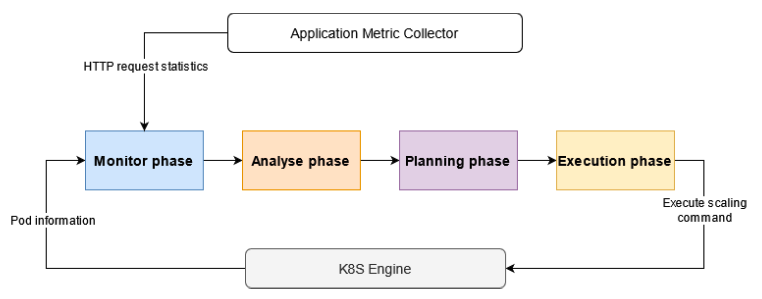
\includegraphics[width=0.8\textwidth]{chapter-2/mape.png}
    \caption{Arsitektur Sistem MAPE, \parencite{riset1}}
    \label{fig:mape}
\end{figure}

\subsection{Penelitian Lainnya}

Adapun \textit{autoscaler} yang sudah dikembangkan dan dibahas di banyak penelitian lain. Pendekatan dan metode yang digunakan sangat variatif. Gambaran umum mengenai penelitian lain yang berhubungan dengan \textit{autoscaler} menggunakan model prediksi, \textit{threshold} atau \textit{rule based} maupun \textit{machine learning} bisa dilihat pada tabel \ref{tab:overview-autoscaler}.

\begin{longtable}{|p{2in}|c|p{1in}|c|p{0.8in}|}

    \caption{Tabel Penelitian Lain terkait Pengembangan Metode \textit{Autoscaling}} \label{tab:overview-autoscaler} \\

    \hline
    \rowcolor{gray!30}\multicolumn{1}{|c|}{\textbf{Paper}} & \textbf{Virtualisasi} & \multicolumn{1}{|c|}{\textbf{Metrik}} & \textbf{Pendekatan} & \multicolumn{1}{|c|}{\textbf{Metode}} \\
    \hline
    \endfirsthead
    %
    \endhead
    %
    \textit{Intelligent Workload Factoring for a Hybrid Cloud Computing Model}, \parencite{zhang} & VM & \textit{Request Rate} & Reaktif & ARIMA \tabularnewline

    \textit{Autonomic Vertical Elasticity of Docker Containers with Elasticdocker}, \parencite{al2017autonomic} & \textit{Container} & Prosesor, Memori & Reaktif & \textit{Rule-based} \tabularnewline

    \textit{Horizontal Pod Autoscaler}, \parencite{hpa2} & \textit{Container} & Prosesor & Reaktif & \textit{Rule-based} \tabularnewline

    \textit{A Novel Resource Prediction and Provisioning Scheme in Cloud Data Center}, \parencite{rpps} & \textit{Container} & Prosesor & Proaktif & ARMA \tabularnewline

    \textit{Workload Prediction Using ARIMA Model and Its Impact on Cloud Applications QoS}, \parencite{workloadprediction} & VM & \textit{Request Rate} & Proaktif & ARIMA \tabularnewline

    \textit{Resource Elasticity Controller for Docker-based Web Applications}, \parencite{resourceelasticity} & \textit{Container} & \textit{Request Rate} & Proaktif & ARIMA \tabularnewline

    \textit{Combining Time Series Prediction Models using Genetic Algorithm to Autoscaling Web Applications Hosted in the Cloud Infrastructure}, \parencite{tspwithga} & - & \textit{Request Rate} & Proaktif & \textit{Genetic Algorithm} \tabularnewline

    \textit{Predicting Cloud Resource Provisioning using Machine Learning Techniques}, \parencite{predictcloudrsrc} & - & \textit{Task Length} & Proaktif & \textit{Artificial Neural Network} \tabularnewline

    \textit{Auto-scaling Microservices on IaaS under SLA with Cost-Effective Framework}, \parencite{asmicrocosteff} & VM & \textit{Request Rate} & Proaktif & \textit{Artificial Neural Network}, \textit{Recurrent Neural Network} \tabularnewline

    \textit{Machine Learning-based Auto-scaling for Containerized Applications}, \parencite{mlbasconapps} & \textit{Container} & \textit{Request Rate} & Proaktif & LSTM \tabularnewline

    \textit{Adaptive Horizontal Scaling of Microservices using Bi-LSTM}, \parencite{adaptivehsmicro} & \textit{Container} & Prosesor, Memori & Gabungan & Bi-LSTM \tabularnewline

    \hline
\end{longtable}

% \section{\textit{Information Retrieval}}
\textit{Information Retrieval} (IR) adalah proses mencari bahan, biasanya berbentuk dokumen, yang bersifat tak terstruktur, biasanya teks, yang memenuhi kebutuhan informasi dari dalam koleksi besar \parencite{inforetrieval}. IR saat ini sangat sering dilakukan contohnya dalam pencarian informasi berkaitan dengan representasi, penyimpanan, pengaturan, dokumen, halaman web, katalog online, catatan, dan objek multimedia. 

Tujuan utama dari IR adalah penyediaan akses yang efektif dan efisien ke informasi yang dibutuhkan oleh pengguna dalam situasi tertentu. Pengguna IR dapat beragam seperti individu, organisasi, maupun sistem yang membutuhkan informasi yang relevan. IR melibatkan penggunaan teknik-teknik seperti \textit{indexing, searching, retrieval,} dan \textit{evaluation} untuk memastikan informasi yang dihasilkan relevan, tepat, dan sesuai dengan kebutuhan pengguna.

Biasanya IR tersusun oleh beberapa komponen, diantaranya.
\begin{enumerate}
    \item \textit{Indexing}, proses mengubah dokumen menjadi bentuk yang lebih mudah dicari oleh sistem IR.
    \item \textit{Searching}, proses pencarian yang dilakukan oleh pengguna dengan memberikan \textit{query} ke dalam sistem IR dan sistem memberikan keluaran berupa dokumen yang paling relevan.
    \item \textit{Retrieval}, proses sistem IR mengambil dokumen yang relevan dan mengurutkan dokumen berdasarkan kesesuaian dengan \textit{query}.
    \item \textit{Evaluation}, proses penilaian kualitas sistem IR yang biasanya mencakup metrik evaluasi seperti \textit{precision}, \textit{recall}, dan skor F1. 
\end{enumerate}

Dalam melakukan proses-proses tersebut, komponen tersebut menggunakan beberapa teknik, diantaranya.
\begin{enumerate}
    \item \textit{Term Weighting}, teknik pemberian bobot terhadap kata-kata untuk membedakan yang lebih penting dan yang kurang.
    \item \textit{Query Expansion}, teknik menambahkan kata-kata yang relevan pada \textit{query} pengguna untuk meningkatkan akurasi hasil pencarian.
    \item \textit{Clustering}, teknik mengelompokkan dokumen yang mirip untuk memudahkan pengambilan.
\end{enumerate}

% \section{Apache Lucene}
Apache Lucene adalah sebuah perpustakaan atau library open-source untuk Information Retrieval (IR) atau pencarian informasi yang berbasis teks. Lucene adalah \textit{library search engine} yang berkinerja tinggi dan berfitur lengkap. Lucene cocok untuk aplikasi yang memerlukan pencarian terstruktur, pencarian teks lengkap, pencarian pada graf dengan banyak node maupun vektor derajat tinggi, koreksi ejaan, atau saran kueri \parencite{apachelucene}. Lucene dikembangkan di bahasa pemrograman Java dan berfokus pada pencarian teks di dalam dokumen.

Lucene menggunakan model inverted index untuk mempercepat proses pencarian. Model ini mengubah dokumen yang diberikan menjadi indeks kata kunci atau \textit{term} dan menunjukkan letak setiap kata kunci tersebut muncul dalam dokumen. Indeks akan digunakan oleh Lucene untuk mencari kata kunci tertentu dalam dokumen dengan sangat cepat.

% \section{\textit{Inverted Index}}
\label{sec:invertedindex}

\textit{Inverted Index} merupakan struktur data yang biasa digunakan untuk mesin pencari \parencite{invertedindex2}. Tujuan dari implementasi struktur data ini pada mesin pencari adalah untuk mengoptimalkan kecepatan query dalam mencari dokumen yang mengandung kata kunci tertentu. Struktur data ini melakukan pemetaan terhadap kata dan kumpulan tupel yang berisikan \textit{identifier} (ID) dokumen dan posisi karakter \parencite{invertedindex}. Struktur data ini biasanya dipakai untuk menggantikan \textit{Forward Index}. \textit{Forward Index} adalah struktur data yang menyimpan seluruh kata dalam sebuah dokumen sehingga jika \textit{forward index} di-\textit{query}, maka akan memerlukan iterasi sekuensial pada setiap dokumen dan kata kunci untuk membuktikan dokumen relevan. Sumber daya waktu, memori, dan pemrosesan yang dibutuhkan untuk melakukan query semacam itu tidak realistis dan praktis karena nyatanya, mesin pencari harus melakukan hal tersebut ke ratusan hinga jutaan dokumen. Dengan inverted index yang dibuat, query dapat diselesaikan dengan cara langsung melompat ke \textit{identifier} (ID) kata kunci melalui \textit{random access} pada inverted index untuk mendapatkan \textit{identifier} (ID) dokumen dan posisi karakter.

% \section{\textit{Elastic Search}}
% \textit{Elastic Search} adalah aplikasi mesin pencarian RESTful.  \textit{Elastic Search} diciptakan sebagai pembungkus dan inovasi dari Apache Lucene yang sekedar hanya \textit{library} karena aplikasi yang beredar saat ini tidak hanya dibuat di atas Java dan membutuhkan fleksibilitas yang tinggi, sedangkan, Apache Lucene terkenal sangat sulit untuk orang awam yang tidak memahami istilah-istilah dan \textit{information retrieval}. \textit{Elastic Search} sendiri dibuat menggunakan Java namun menggunakan \textit{Application Programming Interface} RESTful melalui protokol HTTP sehingga aplikasi dengan bahasa apapun dapat dengan mudah menggunakan aplikasi ini. Tidak hanya itu, API dari \textit{Elastic Search} ini juga sudah sangat dipermudah sehingga pemakai tidak perlu mengetahui istilah-istilah dalam Apache Lucene. Sehingga, \textit{Elastic Search} ini sangat dekat dengan proses umum pada data seperti menyimpan, membaharui, menghapus, pengindeksan, pencarian, dan sebagainya.

\textit{Elastic Search} merupakan sebuah perangkat lunak \textit{open-source} yang ditulis menggunakan bahasa pemrograman Java. \textit{Elastic Search} dibangun di atas Apache Lucene. \textit{Elastic Search} menyimpan data secara terpusat untuk pencarian secepat kilat dan relevan \parencite{elasticsearchorigin}. Selain Apache Lucene, \textit{Elastic Search} memanfaatkan teknologi-teknologi lain untuk meningkatkan fungsionalitas dan kinerja, seperti Apache Hadoop untuk big data processing, Apache Spark untuk data analytics, dan Apache Storm untuk real-time stream processing.

\textit{Elastic Search} didesain sebagai sebuah sistem terdistribusi, yang berarti data yang disimpan pada \textit{Elastic Search} akan didistribusikan ke beberapa \textit{node} atau lebih dikenal sebagai \textit{sharding}, sehingga memungkinkan untuk meningkatkan kinerja, skalabilitas, dan ketahanan pada sistem. Sistem terdistribusi pada \textit{Elastic Search} dapat diatur dan dikonfigurasi agar dapat dijalankan pada beberapa \textit{node} yang terpisah atau pada \textit{cluster} yang terhubung, yang memungkinkan pengguna untuk menyimpan data yang sangat besar dan menjalankan query secara paralel pada beberapa node pada waktu yang bersamaan.

\textit{Elastic Search} dibuat untuk memudahkan pengguna mengakses data dan melakukan pencarian pada data yang besar dan kompleks dengan cepat dan efisien. Meskipun Apache Lucene telah menyediakan fitur-fitur yang bagus untuk \textit{indexing} dan \textit{searching}, tetapi Apache Lucene lebih fokus pada teknologi inti dan pengembangan secara \textit{information retrieval} seperti mengoptimisasi dan pengembangan \textit{indexing} dan \textit{searching}. Hal tersebut menyebabkan penggunaan Lucene memerlukan banyak pengaturan dan konfigurasi tambahan untuk bisa diintegrasikan dengan aplikasi yang lebih besar. Dalam hal ini, \textit{Elastic Search} hadir sebagai sebuah solusi yang lebih terintegrasi, mudah digunakan, dan dapat diatur secara fleksibel. \textit{Elastic Search} memanfaatkan Lucene sebagai mesin pencari, tetapi menambahkan banyak fitur-fitur dan fungsionalitas tambahan untuk meningkatkan kinerja dan kemudahan penggunaan. Selain itu, \textit{Elastic Search} dirancang sebagai aplikasi dengan sistem terdistribusi dan \textit{scalable} yang memungkinkan data terdistribusi di beberapa node atau \textit{sharding}, sehingga memungkinkan \textit{Elastic Search} untuk mengatasi masalah data yang sangat besar dan kompleks secara efektif dan efisien. Sedangkan, Lucene hanya pada batas kakas atau \textit{library}.

\textit{Elastic Search} dapat digunakan dengan protokol HTTP dan REST API. Dalam penggunaan dengan protokol HTTP, \textit{Elastic Search} menyediakan endpoint API RESTful HTTP yang dapat diakses oleh pengguna dengan memakai klien HTTP, seperti perintah cURL, \textit{Postman} atau \textit{web browser}. Pengguna dapat membuat permintaan HTTP seperti GET, POST, PUT, DELETE ke API endpoint melalui klien HTTP, dan \textit{Elastic Search} akan memberikan respon sesuai dengan permintaan.

Dalam \textit{Elastic Search} terdapat beberapa operasi yang dapat dilakukan, diantaranya:
\begin{enumerate}
    \item \textbf{\textit{Index}}
    
    Operasi ini akan dijelaskan secara khusus pada bagian selanjutnya, \ref{sec:index}.

    \item \textbf{\textit{Get}}
    
    Operasi \textit{Get} digunakan untuk mengambil dokumen individual berdasarkan ID-nya dari indeks tertentu.
    
    \item \textbf{\textit{Query}}
    
    \textit{Query} digunakan untuk melakukan pencarian dan pengambilan data yang sesuai dengan kriteria tertentu. \textit{Elasticsearch} menyediakan berbagai jenis query seperti pencarian teks lengkap, pencocokan kata kunci, pencocokan frasa, pencarian fuzzy, dan lain-lain.
    
    \item \textbf{\textit{Fetch}}
    
    \textit{Fetch} adalah proses pengambilan dokumen lengkap dari indeks setelah melakukan query. Saat ditemukan, \textit{Elasticsearch} mengambil dokumen dari indeks dan akan digunakan sebagai respon kepada pengguna.
    
    \item \textbf{\textit{Scroll}}
    
    \textit{Scroll} adalah mekanisme pengambilan dokumen yang banyak dari hasil pencarian tanpa perlu mengirimkan \textit{query} ulang. Hal ini menyebabkan pengambilan dokumen dapat menjadi lebih efisien dalam beberapa permintaan, namun, dalam beberapa kasus, bisa menjadi lebih lama untuk mengambil semua dokumen yang relevan.
    
    \item \textbf{\textit{Suggest}}
    
    \textit{Suggest} adalah mekanisme untuk memberikan saran atau \textit{autocompletion} saat pengguna memasukkan kata kunci atau frasa. Biasanya digunakan untuk \textit{autocompletion}, pengoreksi kesalahan pengejaan, dan saran pencarian lainnya.
    
    \item \textbf{\textit{Bulk}}
    
    \textit{Bulk} adalah operasi yang digunakan untuk memasukkan atau memperbarui beberapa dokumen dalam satu permintaan.
    
    \item \textbf{\textit{Flush}}
    
    \textit{Flush} adalah operasi yang digunakan untuk mengosongkan memori \textit{cache} dan menulis data yang tertunda ke disk. Operasi ini memastikan bahwa data yang ditulis telah disimpan secara permanen di indeks.
    
    \item \textbf{\textit{Refresh}}
    
    \textit{Refresh} adalah operasi yang digunakan untuk membuat perubahan yang terjadi pada indeks secara terlihat dan dapat dicari. Saat melakukan operasi indeks seperti menambahkan atau menghapus dokumen, perubahan tersebut tidak langsung terlihat oleh pencarian hingga dilakukan operasi refresh.
\end{enumerate}

% \section{Java \textit{Virtual Machine}}
\textit{Java Virtual Machine} atau JVM adalah program yang dapat membaca program java yang telah dikompilasi atau biasa dikenal sebagai \textit{java bytecode} dan menginterpretasikannya menjadi bahasa mesin yang dapat dieksekusi oleh komputer \parencite{java12}. Secara tidak langsung, JVM merupakan komponen utama dalam menjalankan program bahasa Java. Struktur JVM terdiri dari \textit{runtime data structure} di memori dan dua subsistem yang berhubungan langsung dengan \textit{runtime data structure} yaitu \textit{class loader} dan \textit{execution engine}. Semua program yang dibuat dengan Java akan dikompilasi ke \textit{java bytecode} yang nantinya akan diinterpretasikan oleh JVM untuk dieksekusi komputer.

\textit{Elastic Search}, yang terbuat dari bahasa Java, berjalan di atas platform Java Virtual Machine (JVM). JVM sendiri akan bertanggung jawab untuk menjalankan kode Java dan mengelola sumber daya yang dibutuhkan oleh program, seperti memori, prosesor, dan jaringan. Sehingga, JVM memiliki peran penting dalam menjalankan \textit{Elastic Search} dan memastikan kinerjanya baik. JVM menyediakan opsi pengaturan yang membuat pengguna dapat mengontrol alokasi memori dan penggunaan CPU pada aplikasi \textit{Elastic Search}. Dengan mengatur parameter JVM yang tepat, pengguna dapat memperbaiki kinerja \textit{Elastic Search} dan memaksimalkan penggunaan sumber daya sistem.

Parameter yang berhubungan erat dengan alokasi sumber daya pada \textit{Elastic Search} dan mempengaruhi kinerja JVM adalah parameter \textit{heap size} (-Xms dan -Xmx) yang mengatur ukuran \textit{heap memory} yang dialokasikan untuk JVM. \textit{Heap memory} adalah tempat JVM menyimpan objek dan data dari aplikasi Java yang sedang berjalan. Parameter -Xms menentukan ukuran \textit{heap memory} awal yang dialokasikan ketika JVM dimulai, sedangkan parameter -Xmx menentukan batas maksimal ukuran \textit{heap memory} yang dapat dipakai oleh JVM. Selain itu, terdapat parameter lain yang dapat mempengaruhi kinerja JVM dan \textit{Elastic Search}, seperti \textit{thread pool size}, \textit{circuit breaker settings}, dan lain-lain. Parameter-parameter ini dapat diatur melalui file konfigurasi \textit{Elastic Search} atau melalui command line arguments saat menjalankan \textit{Elastic Search}.

% \section{\textit{Indexing}}
\label{sec:index}

\textit{Indexing} adalah suatu teknik untuk menyusun kata-kata dan mengurangi usaha untuk mencari hal yang berkaitan dengan kata tersebut jika diperlukan, \parencite{database}. Secara umum, indeks banyak digunakan pada buku teks, basis data, dan sistem information retrieval. Seperti salah satu contoh tekniknya adalah \textit{Inverted Index} yang telah dijelaskan pada \ref{sec:invertedindex}.

Terdapat kelebihan penggunaan indeks, diantaranya:
\begin{enumerate}
    \item \textit{Indexing} dapat mempercepat proses pencarian data dengan membuat indeks dan mencocokkan kata kunci dengan indeks tersebut, sehingga mesin dapat menemukan data dengan lebih cepat.
    \item \textit{Indexing} dapat meningkatkan akurasi pencarian dengan menampilkan hasil pencarian yang lebih relevan dengan kata kunci yang dimasukkan.
\end{enumerate}

Namun, ada juga kelemahan dari penggunaan indeks, yaitu sebagai berikut.
\begin{enumerate}
    \item \textit{Indexing} memerlukan ruang penyimpanan tambahan untuk membuat indeks.
    \item Proses pembuatan \textit{indexing} memerlukan waktu, terutama jika data yang akan di-indeks sangat banyak.
\end{enumerate}

Sehingga, dapat disimpulkan penggunaan indeks sangat bermanfaat namun menambahkan biaya.
Pada kasus-kasus dokumen besar, penggunaan indeks pengaruhnya sangat besar karena mesin akan mencari data pada indeks terlebih dahulu sebelum mencari data pada dokumen asli. Hal ini dapat membantu mengurangi waktu pencarian dan menghemat penggunaan memori karena mesin tidak perlu membaca seluruh dokumen untuk menemukan data yang dicari. Namun, apabila \textit{indexing} dilakukan secara berlebihan, akan terdapat banyak indeks yang tidak terpakai dan hanya akan menambah kebutuhan memori.

% Konsep \textit{caching} sendiri adalah menyimpan data yang sering diakses pada level cache atau memori yang lebih dekat dengan CPU agar dapat diakses dengan cepat saat ingin melakukan pencarian, lihat gambar \ref{fig:cache-level}. \textit{Cache} sendiri biasanya memiliki ruang yang terbatas sehingga biasanya membuang data yang sudah tidak diakses sehingga jika dibutuhkan harus dicari ke \textit{storage}. Konsep ini ditiru oleh basis data dan aplikasi \textit{information retrieval} untuk mempercepat proses pencarian dengan memanfaatkan \textit{indexing} untuk mencari (lihat gambar \ref{fig:cache-app}) dan \textit{caching} untuk mengembalikan data yang sering diakses dengan memanfaatkan memori.

% \begin{figure}[h]
%     \centering
%     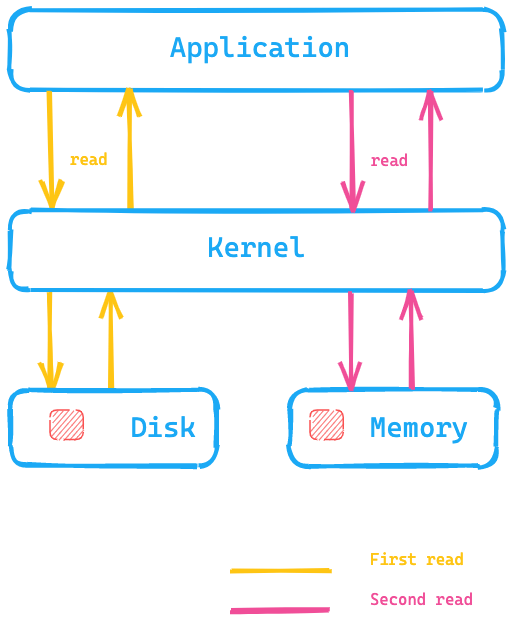
\includegraphics[width=0.5\textwidth]{chapter-2/cache-app.png}
%     \caption{Prinsip Cache pada Aplikasi}
%     \label{fig:cache-app}
% \end{figure}

% \begin{figure}[h]
%     \centering
%     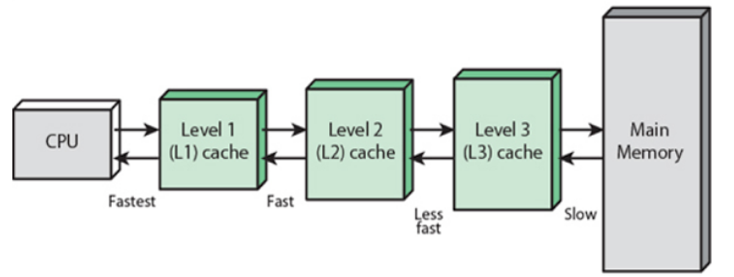
\includegraphics[width=0.5\textwidth]{chapter-2/cache-memory.jpeg}
%     \caption{Level-level pada Cache}
%     \label{fig:cache-level}
% \end{figure}

% \section{\textit{Caching}}
\textit{Caching} adalah teknik menyimpan data atau informasi yang sering digunakan secara lokal pada suatu tempat agar dapat diakses lebih cepat kedepannya. \textit{Caching} dapat digunakan untuk menyimpan hasil pencarian yang sering dilakukan oleh pengguna, sehingga jika pengguna melakukan pencarian yang sama, hasilnya dapat diambil dari \textit{cache} yang tersimpan dan tidak perlu melakukan pencarian.

Terdapat relevansi \textit{caching} dengan indeks, \textit{caching} dapat membantu meningkatkan kinerja sistem indeks dengan menyimpan hasil pencarian yang sering dilakukan dan mengaksesnya dari \textit{cache} saat pengguna melakukan pencarian yang sama. Dengan demikian, waktu dan sumber daya yang diperlukan untuk memproses pencarian dapat dihemat. Pengguna juga dapat mengakses hasil pencarian dengan lebih cepat karena data yang dicari sudah disimpan di \textit{cache} dan tidak perlu memproses ulang dari indeks. Namun, perlu diingat bahwa ukuran cache harus dibatasi, sehingga \textit{caching} tidak menggunakan memori secara berlebihan.

% \input{chapters/chapter-2/15-simulasi}
% \section{Pembelajaran Mesin}
% Pembelajaran Mesin adalah sebuah bidang pembelajaran yang mempelajari pemahaman dan membangun metode untuk "belajar" dengan memanfaatkan data untuk meningkatkan banyak aspek terutama efisiensi dan kualitas terhadap suatu rangkaian tugas. Algoritma pembelajaran mesin membangun model berdasarkan data sampel yang biasa disebut \textit{training data} untuk menghasilkan model yang dapat memprediksi atau membuat keputusan tanpa diprogram secara eksplisit, \parencite{ml}.

% \subsection{\textit{Reinforcement Learning}}
% \textit{Reinforcement learning} atau RL adalah bidang pembelajaran mesin yang mengotomasi sebuah agen untuk mengambil tindakan dan memaksimalkan \textit{reward} dari aksi yang dilakukan, \parencite{reinforcementlearning}. RL adalah salah satu paradigma dari tiga pembelajaran mesin dasar seperti \textit{Supervised Learning} dan \textit{Unsupervised Learning}. Singkatnya, RL membuat agen dapat mengoreksi pengetahuannya secara terus menerus agar dapat memaksimalkan fungsinya. Berbeda dengan \textit{Supervised Learning}, RL tidak memerlukan label dan tidak memerlukan secara eksplisit dikoreksi. Fokus dalam membangun RL, adalah mencari keseimbangan eksplorasi terhadap lingkungan baru dan eksploitasi terhadap pengetahuan yang dimiliki.

% penelitian terkait